% Chapter Template

\chapter{Performance and Transferability of DBM: Reverse-mapping of Syndiotactic Polystyrene} % Main chapter title
\label{bm_ps} % Change X to a consecutive number; for referencing this chapter elsewhere, use \ref{ChapterX}

In this chapter, deepbackmap (DBM) is applied to a challenging condensed-phase polymeric system that consists of syndiotactic polystyrene (sPS). The performance of DBM is analyzed in terms of three important aspects: 1) The general reverse-mapping capability of the model is probed, i.e. the ability to reproduce a reference all-atom (AA) distribution from coarse-grained (CG) configurations. 2) The transferability of the model across different thermodynamic state points is tested. To this end, DBM is trained solely on data obtained in a high-temperature melt and the model's transferability to lower temperatures, where the system is in a crystalline state, is probed. 3) The transferability of DBM across chemical space is examined. In particular, DBM is trained on liquids of small molecules. After training, the model is transferred to the more challenging polymeric system of sPS. 

This chapter presents content that has been previously published in the following research articles \cite{stieffenhofer2020adversarial, stieffenhofer2021adversarial}. The content is reproduced here with kind permission from the other authors and the journals which published
these articles.

\begin{figure}
  \centering
  \captionsetup{width=1.0\linewidth}
      \includegraphics[width=0.70\textwidth]{./Figures/adversarial_backmapping/intro.pdf}
  \caption{CG (left) and AA (right) representation of sPS. The CG monomer consists of two beads, denoted $A$ for the chain backbone and $B$ for the phenyl ring. Reprinted from \cite{stieffenhofer2020adversarial}.}
  \label{FIG:sPS_single_chain}
\end{figure}

\newpage
\hfill \break
\noindent \textit{Marc Stieffenhofer, Michael Wand, Tristan Bereau}\\
\textbf{Adversarial reverse mapping of equilibrated condensed-phase molecular structures}\\
Machine Learning: Science and Technology, Volume 1, Number 4\\
DOI: 10.1088/2632-2153/abb6d4\\
$\copyright$ IOP Publishing Ltd, 2020
\hfill \break

\noindent \textit{Marc Stieffenhofer, Tristan Bereau, Michael Wand}\\
\textbf{Adversarial reverse mapping of condensed-phase molecular structures: Chemical transferability}\\
APL Materials 9, Volume 9, Number 3\\
DOI: 10.1063/5.0039102\\
$\copyright$ AIP Publishing LLC, 2021
\hfill \break

\section{Set-up and Reference Data}

In this section, the reference data used to train and evaluate the performance of DBM is introduced. In addition, a baseline method is utilized to compare the results of DBM with a backmapping method frequently used in the multiscale modeling community. 

\subsection{Syndiotactic Polystyrene}
\label{SEC:sPS}

Polystyrene (PS) is an aromatic polymer made from the monomer styrene, which is an organic compound consisting entirely of carbon and hydrogen. Physical and chemical properties of PS depend significantly on its tacticity, i.e. the arrangement of the phenyl groups along the polymer backbone. In this study, syndiotactic polystyrene (sPS) is used, where the phenyl groups are arranged on alternating sides of the polymer backbone. An illustration of a single polymer chain with AA as well as CG resolution is shown in Fig. \ref{FIG:sPS_single_chain}. 

Despite its simple chemical structure, sPS displays a rich conformational space and exhibits complex polymorphic behavior. As such, sPS is a well suited candidate to study the transferability properties of DBM. Upon thermal annealing, the sPS melt undergoes a phase transition from amorphous to a crystalline phase at $T \approx 450$~K \cite{liu2018polymorphism}. Five different crystalline forms of sPS have been reported experimentally. Here, the focus is set on the $\alpha$ and $\beta$ polymorphs, which are illustrated in Fig. \ref{FIG:sPS_polymorphs}.

The atomistic data in this study is reported in Liu \emph{et al.} \cite{liu2018polymorphism}; the underlying force field is based on the work of Mueller-Plathe \cite{muller1996local}. The system is sampled using Replica Exchange MD simulations, which are performed using the molecular dynamics package {\sc GROMACS} 4.6 \cite{hess2008gromacs}. The simulations are carried out in the $NPT$ ensemble using the velocity rescaling thermostat and the Parrinello-Rahman barostat. An integration time step of $1$~fs is used. For additional details regarding the simulations, the reader is referred to the work of Liu \emph{et al.} \cite{liu2018polymorphism}.

Pairs of corresponding AA and CG snapshots are generated by mapping AA configurations onto the CG resolution. Three data sets are constructed from uncorrelated snapshots selected from different trajectories simulated at $T = 313$~K, $453$~K, and $568$~K. To cover a wide range of conformational space, each atomistic simulation was initialized from a different structure: The simulation at $313$~K started from a $\beta$ structure, at $453$ K from an $\alpha$ structure and at $568$~K from an amorphous configuration. The system includes $36$ polystyrene chains and each chain consists of $10$ monomers. Each data set contains $12$ snapshots for training and $78$ snapshots for testing.

The fine-to-coarse mapping is based on the CG model developed by Fritz \emph{et al.} \cite{fritz2009coarse}. Each monomer is mapped onto two beads of different types, denoted $A$ for the chain backbone and $B$ for the phenyl ring (see Fig. \ref{FIG:sPS_single_chain}). Bonds are formed only between backbone and phenyl ring beads, i.e. the CG polymer is represented as a linear chain $A$-$B$-$A$-$B\cdots$. The close connection between backbone beads $A$ is reproduced indirectly by angular potentials. While the CG model is parameterized in the melt, Liu \emph{et al.} have shown that it is transferable to the crystalline phase, where it stabilizes the experimentally observed $\alpha$ and $\beta$ polymorphs \cite{liu2018polymorphism}. 

%In isotactic PS the phenyl groups are positioned on the same side of the polymer chain, while in syndiotactic PS the phenyl groups are arranged on alternating sides of the chain. In atactic PS the phenyl groups are arranged randomly. 

\subsection{Octane and Cumene}
\label{SEC:Oct_Cum}

Octane and cumene are small hydrocarbons. While octane is an acyclic alkane, cumene is aromatic. MD simulations of octane and cumene liquids are performed using the molecular dynamics package {\sc GROMACS} 5.0 \cite{hess2008gromacs}. The GROMOS force field is used and topologies are generated by {\sc Automated Topology builder} \cite{malde2011automated}. Note that the GROMOS and sPS force fields differ in parameterization strategies. While both force fields aim at reproducing thermodynamic properties, the GROMOS force field is designed for a broad range of chemistries, while the parametrization for sPS is custom-built from a specific force field designed for benzene. This leads to evident differences in force field parameters, especially in terms of the non-bonded Lennard-Jones interactions and partial charges.

The simulation boxes of octane and cumene contain 215 and 265 molecules, respectively. MD simulations are performed in the $NPT$ ensemble using the velocity rescaling thermostat and the Parrinello–Rahman barostat. The integration time step is set to 1~fs and both systems are sampled at $350$~K.

As illustrated in Fig. \ref{FIG:cheh_trans_intro}, the fine-to-coarse mapping is based on the mapping for sPS. Cumene is mapped onto one bead of type $B$ for the phenyl ring and two beads of type $A$ for the backbone, each containing a methyl group and sharing the $CH$ group connected to the phenyl ring. Octane is mapped onto four beads of type $A$, where neighboring $A$ beads share a $CH_{2}$ group.

\subsection{Baseline Method}

The results of DBM are compared to a generic backmapping strategy, as described in Sec. \ref{SEC:bm_generic}. Specifically, the backmapping script developed by Wassenaar \emph{et al.} is utilized \cite{wassenaar2014going}. In a first step, this method places each particle on the weighted average position of the CG beads it corresponds to and optionally adds a random displacement. In addition, the protocol allows the user to apply geometric modifiers setting the alignment of the next particle "cis", "trans", "out", or "chiral" with respect to the other particles. The modifiers are crucial for the performance of this method and require a careful adjustment by the user.

After the initial structure is generated, the protocol by Waasenaar \emph{et al.} continues with multiple cycles of force field based energy minimization for relaxation. Here, the first cycle consists of $200$ steps and takes only bonded interactions into account. Afterwards, all interactions are turned on and energy minimization continues with a total number of $5000$ steps. The original protocol continues with several cycles of position restrained MD simulations to equilibrate the relaxed system. However, comparing DBM with such equilibrated backmapped structures is not insightful, since applying MD simulations would evidently reproduce the Boltzmann distribution, which is already captured by the reference test set. In order to highlight the capability of DBM to generate equilibrated molecular structures without MD, the script by Waasenaar \emph{et al.} is stopped after the relaxation, such that reconstructions generated by DBM can be compared to energy-minimized configurations prior to MD.

%DBM aims at generating molecular structures without relying on further MD simulations.
\subsection{Specifications of DBM}
\label{DBM_specifications}

DBM deploys a convolutional neural network (CNN) architecture with residual connections for the generator $g$ and critic $c$ \cite{he2016deep}. A detailed description of the network architecture can be found in Fig.~A.\ref{APPENDIX:DBM_architecture} in the appendix. Training is performed using the Adam optimizer \cite{kingma2014adam}. The cutoff distance applied for the local environments is set to $r_{\text{cut}} = 1.2$ nm. To prevent numerical instabilities in the beginning of the training, the prefactor for the regularization term based on the potential energy is set initially to $\lambda_{\text{pot}}= 0$ and increased smoothly to $\lambda_{\text{pot}} = 0.01$. The prefactor scaling the weight of the gradient penalty term is set to $\lambda_\textup{gp} = 0.1$ throughout the training. To obtain reliable gradients for the generator $g$, the critic $c$ is trained five times in each iteration while the generator $g$ is trained once.

The autoregressive approach of DBM is prone to accumulate errors, i.e. misplaced atoms can hinder $g$ to find suitable positions for subsequent atoms. As a remedy, the potential energy is used during inference in order to spot and reject outliers. For each local environment, a mini-batch is constructed by random rotations around the director axis (see Sec. \ref{DBM:loc_env}). Since the CNN architecture is not rotational equivariant, predictions will slightly differ depending on the relative orientations. In addition, different prior samples $\mathbf{z}$ are used for each element in the mini-batch to further increase variations of generated structures. As a straight-forward solution to mitigate the effect of misplaced atoms, the structure with the lowest potential energy is selected from the generated ensemble. While this simple procedure performs well in practice, it should be noted that it might introduce a bias towards low-energy structures. In addition, hydrogens are removed from the current and adjacent beads for the reconstruction of heavy atoms, such that misplaced hydrogens do not affect the positioning of heavy atoms.

\section{General Performance}
\label{SEC:DBM_general_performance}

In this section, the general performance of DBM is probed. To this end, DBM is trained on the high-temperature data set at $568$~K, where the sPS system is in a melt state. After training, the model is applied to test data, i.e. hold-out data at the same temperature.   

\subsection{Results}

\begin{figure}
  \centering
  \captionsetup{width=1.0\linewidth}
      \includegraphics[width=1.05\textwidth]{./Figures/adversarial_backmapping/sPS_temp_trans/ff_dists_and_rdf.pdf}
  \caption{ Canonical distributions for various force field interaction terms at (left) $T = 568$~K, (middle) $T = 453$~K and (right) $T = 313$~K for reference structures (black), structures generated with a baseline method based on energy-minimization (red), and the new method DBM (blue). The model is trained solely on the high temperature data (left), but deployed at lower temperatures (middle and right). (a)–(c) C-C-C backbone angle, (d)–(f) C-C-C-C backbone dihedral, (g)–(i) C-C-C-C improper dihedral, (j)–(l) Lennard-Jones energies, and (m)–(o) radial distribution functions, g(r), of the non-bonded carbon atoms. Reprinted from \cite{stieffenhofer2020adversarial}.}
  \label{FIG:sPS_temp_trans_ff_dists}
\end{figure}

Fig. \ref{FIG:sPS_temp_trans_ff_dists} displays distribution functions for several structural and energetic properties of sPS. The distributions of intramolecular carbon backbone angle and dihedral, shown in panels (a) and (d), are in excellent agreement with the reference distributions. On the other hand, structures generated with the baseline method display distributions that are more compressed compared to the reference system, which is expectable from an approach based on energy minimization. As shown in panel (g), the distribution for the carbon improper dihedral of the phenyl group is slightly biased to smaller angles for configurations generated with DBM. However, the small range of angles, imposed by the planarity of the ring, has to be emphasized. The distribution of the baseline method is even more peaked, i.e. fluctuations around the planar structure are significantly suppressed.

A very important aspect towards generating well-equilibrated configurations in a condensed environment is the correct reproduction of Lennard-Jones energies. Panel (j) displays the distribution of Lennard-Jones energies obtained separately for each chain. While structures generated with DBM show slightly too large high-energy tails, the overall match with the reference distribution is remarkably good. The baseline method systematically and drastically over-stabilizes the system. 

Further, the pair correlation function $g(r)$ for non-bonded carbon pairs is analyzed in panel (m). Structures generated with DBM show an excellent agreement with the reference distribution indicating an accurate reconstruction of pairwise distances. The baseline method is also able to generate pair correlations with high accuracy, but still displays some discrepancies to the reference system.

%\subsection{Discussion}

%DBM is an ML approach for the backmapping of CG molecular structures that is capable to operate in a condensed environment. Here, it is applied to melts of sPS at $568$ K. The results are compared with a baseline method based on energy-minimization.

%DBM reproduces structural and energetic properties of the reference system remarkably well. The new method yields well-equilibrated configurations at the high-temperature state point that it was trained on. On the other hand, the energy minimization protocol of the baseline method over-stabilizes the system. As such, further MD simulations controlled by a thermostat would be required to reproduce the local correlations at the particular canonical state point.

\section{Temperature Transferability: From Melt to Crystal}
\label{DBM:temp_trans}

After successfully recovering the state point DBM was trained on, the model's ability to transfer across temperatures is probed. As illustrated in Fig. \ref{FIG:sPS_polymorphs}, the training of DBM is fixed to the high-temperature ensemble, while testing is performed at lower temperatures \textit{without} reparameterization. Specifically, the model is trained at $568$ K and tested at $453$ K and $313$ K. Note that the sPS system undergoes a phase transition at $\approx 450$ K, going from a melt to a crystalline state with different polymorphs. In particular, the test data set contains snapshots of the $\alpha$ and $\beta$ polymorphs that differ in the packing of the sPS chains. 

\begin{figure}
  \centering
      \includegraphics[width=0.6\textwidth]{./Figures/adversarial_backmapping/sPS_temp_trans/ps_polymorphs.pdf}
  \caption{Polymorphism of Polystyrene. At high temperature ($T = 568$ K) the polymeric system is an a melt state. At lower temperatures the CG model mostly stabilizes the $\alpha$ polymorph at $T = 453$ K and the $\beta$ polymorph at $T = 313$ K. DBM is trained solely on the high-temperature ensemble and its transferability to the lower temperatures is probed. Reprinted from \cite{stieffenhofer2020adversarial}.}
  \label{FIG:sPS_polymorphs}
\end{figure}

\subsection{Results}
\label{DBM:sPS_temp_trans}

The transferability of DBM to the crystalline phase of sPS is analyzed in terms of structural and energetic distributions. In addition, a higher-order investigation facilitated by the Sketch-Map (SM) algorithm is performed to obtain a two-dimensional projection of configuration space \cite{ceriotti2011simplifying, tribello2012using}. Finally, AA MD simulations initialized from reference and backmapped structures are evaluated.

\subsubsection{Distributions of Structural and Energetic Features}

Distributions for structural and energetic properties at $453$ K and $313$ K can be found in the middle and right culumn of Fig. \ref{FIG:sPS_temp_trans_ff_dists}, respectively. The reference system displays a number of significant changes upon cooling: distributions of angles become more compressed, the side peak in the backbone dihedral vanishes, the distributions of Lennard-Jones energies are shifted towards lower energies and the pair correlation function of non-bonded carbon atoms is more peaked. 

The ML model adapts remarkably well to the crystalline phase in terms of the angle and dihedral distributions shown in panels (b,c,e,f,h,i): DBM yields distributions that follow the reference distributions and become more compressed upon cooling. Lennard-Jones energies displayed in panels (k) and (l) are also shifted and match with the reference distributions. Moreover, non-bonded pair correlations in the crystalline phase are reproduced with remarkable accuracy, as indicated in panels (n) and (o). 

On the other hand, the baseline method does not adapt well to lower temperatures. Due to the energy minimization, similar distributions are obtained as for the high-temperature data, which becomes especially apparent for the side peak of the backbone dihedral in panels (e) and (f), as well as the flat pair correlation function in panels (n) and (o). 

\subsubsection{Sketch-Map}

\begin{figure}[h]
  \centering
      \includegraphics[width=1.0\textwidth]{./Figures/adversarial_backmapping/sPS_temp_trans/sm_snapshots.pdf}
  \caption{ Two-dimensional projection of the configuration space obtained with SM. Each point represents a sPS chain in a condensed-phase environment at (a) $T = 568$ K, (b) $T = 453$ K and (c) $T = 313$ K. Projections for reference structures (black), backmapped structures obtained with the baseline method (red) and with DBM (blue) are shown. For each panel, snapshots are backmapped from identical CG configurations. A projection of the entire data set is displayed in gray for visual guidance. Reprinted from \cite{stieffenhofer2020adversarial}.}
  \label{FIG:sPS_temp_trans_SM}
\end{figure}

Evaluating large-scale structural features beyond pair-statistics is challenging, since the high dimensionality of the system does not allow to directly visualize the configuration space. For this reason, dimensionality reduction is applied to further examine the model's accuracy at higher order. As explained in Sec. \ref{MS:sketchmap}, linear dimensionality reduction techniques are insufficient in many cases to capture the structure of data obtained from MD trajectories. Therefore, SM is applied to build a two-dimensional map representing proximity relationships between sPS chains \cite{ceriotti2011simplifying, tribello2012using}.

The descriptors for the sPS chains consist of a set of representations for the local environments $\mathcal{H}$ centered around alternating backbone carbon atoms that are directly linked to a phenyl group. The pairwise distance between two such environments is encoded using a similarity kernel $k(\mathcal{H}, \mathcal{H}') = \mathbf{p}(\mathcal{H}) \mathbf{p}(\mathcal{H'})$ based on the normalized many-body smooth overlap of atomic position (SOAP) representation $\mathbf{p}(\mathcal{H})$ \cite{bartok2013representing}. Hydrogen atoms are neglected in the SOAP representation. To compare two sPS chains $a$ and $b$, the covariance matrix 

\begin{equation}
 C_{ij}(a,b) = \mathbf{p}(\mathcal{H}^a_i) \mathbf{p}(\mathcal{H}^b_j)
\end{equation}

is computed, which contains the complete information of the pairwise similarity of all local environments taken into account between the two structures. In order to obtain a global similarity kernel $k(a,b)$, the covariance matrix $C_{ij}(a,b)$ has to be mapped to a single scalar value, which is achieved using a regularized entropy match kernel \cite{de2016comparing}.

Fig. \ref{FIG:sPS_temp_trans_SM} displays the two-dimensional projection obtained with SM, where each point represents a single sPS polymer chain and its local environment. The projection yields a number of distinct clusters. The reference data forms a single cluster at the low-temperature data at $313$ K (panel (c)), which can be associated with the $\beta$ polymorph. The high-temperature data at $568$ K (panel (a)) is mapped to multiple clusters indicating more diversity, i.e. it includes amorphous, $\alpha$ and other structures. The data set at an intermediate temperature of $453$ K (panel (b)) is mapped mostly to the cluster corresponding to the $\alpha$ polymorph, but also contains some amorphous and other structures.

Structures obtained with DBM display a significant overlap with the reference points for all three data sets indicating closeness in configuration space and high fidelity of the backmapped structures. This is in strong contrast to the energy-minimized structures obtained with the baseline method, which map to different areas in the two-dimensional projection of configuration space compared to the reference configurations. 

%Moreover, the baseline method is not able to recover the correct number of clusters for all three temperatures highlighting a lack of temperature sensitivity.
\subsubsection{MD Simulation}

Backmapped structures that serve as a starting point for further MD simulations typically require lengthy preparations, such as energy minimization, temperature ramp up phase and thermostat/barostat equilibration. In the following, the high quality of backmapped structures obtained with DBM is demonstrated by running MD simulations \textit{without} any heat-up.

The simulations are carried out in the $NPT$ ensemble using the velocity rescaling thermostat and the Parrinello-Rahman barostat. Initial velocities are generated according to a Maxwell distribution and an integration timestep of $1$ fs is used. 

Fig. \ref{FIG:sPS_eq} displays the time evolution of the potential energy during the simulations at (a) $T = 313$ K and (b) $T = 568$ K. Simulations starting from reference or backmapped structures obtained with DBM show a similar evolution of the potential energy at both temperatures and reach a steady value after $\approx 100$ ps. On the other hand, simulations starting from backmapped structures obtained with the baseline method show a different behavior: The potential energy of simulations performed at $313$ K settles at significantly higher energies compared simulations starting from reference or DBM structures. This indicates poorly initialized structures that get trapped into local minima with high energy barriers. However, this issue is not apparent at $568$ K, where all simulations display a similar behavior independent of their initialization. This can be rationalized with the higher temperature that increases the probability of escaping local minima. 

\begin{figure}
  \centering
  \captionsetup{width=1.0\linewidth}
      \includegraphics[width=1.0\textwidth]{./Figures/adversarial_backmapping/sPS_temp_trans/eq.pdf}
  \caption{Evolution of the potential energy in MD simulations without heat-up starting from reference structures (black), backmapped structures obtained with the baseline method (red) and with DBM (blue). Reprinted from \cite{stieffenhofer2020adversarial}.}
  \label{FIG:sPS_eq}
\end{figure}

%\subsection{Discussion}

%In this section, the temperature transferability of DBM is probed. While the training is fixed to melt configurations at a high temperature, the model is deployed at lower temperatures, where the sPS system is in a crystalline state. DBM retains the excellent performance it has shown for the high temperature state point and reproduces the reference distributions in the crystalline state with remarkable accuracy. A higher-order investigation, facilitated by the SM algorithm, further emphasizes the structural accuracy. In addition, MD simulations initialized from backmapped structures display a similar behavior as simulations initialized from reference structures. In summary, the model is able to reproduce local correlations at different state points than it was trained on. 

%This is in strong contrast to the baseline method, which lacks temperature sensitivity due to the energy minimization. Moreover, it is demonstrated that performing MD simulations initialized from backmapped structures from the baseline method is challenging in the crystalline state, as the system evidently gets stuck in local minima. As such, human intervention would be required to achieve proper equilibration, which hinders the automation of such processes.

%The remarkable transferability features of DBM can be rationalized in terms of a scale-separation: The model learns to reproduce well-equilibrated local correlations while large-scale features are dictated by the CG snapshot. As such, the backmapped structure is composed of two sources of information, 1) the learned local features and 2) the CG structure. However, most of the temperature dependence is carried by the latter, as shown by Liu \emph{et al.} that the applied CG model reproduces the crystallization transition remarkably well \cite{liu2018polymorphism}. On the other hand, local features are less temperature sensitive, since they correspond primarily to covalent interactions that operate on energy scales significantly larger than $k_B T$. As such, the local correlations learned in the melt are transferable across a phase transition. However, it is not clear whether the other direction, i.e. training at a low temperature and transferring to a high temperature, would yield satisfactory results. In particular, high temperatures facilitate a broad exploration of configuration space and therefore, some important conformations might be missing when the training would be restricted to a low temperature ensemble. 

\section{Chemical Transferability: From Small Molecules to Polymers}

In this section, the transferability of DBM across chemical space is explored. To this end, the generalization of the model beyond the chemistry used for training is probed by recycling the learned local correlations to make predictions for molecules absent from the training data set. 

DBM uses an sequential approach to reconstruct atomic environments. Further, it is based on a locality assumption, i.e. the placement of one atom is assumed to rely only on short-range force field related features. As such, DBM only learns local correlations while large-scale features are adapted from the CG structure. It can be hypothesized that such local environments strongly overlap across chemical space, and thus, it is likely that small-scale features can be shared between different molecules. This makes DBM a promising candidate toward achieving chemical transferability. 

\begin{figure}
  \centering
  \captionsetup{width=1.0\linewidth}
      \includegraphics[width=1.0\textwidth]{./Figures/adversarial_backmapping/sPS_chem_trans/intro.pdf}
  \caption{AA and CG representations of different molecules. A similar fine-to-coarse mapping is applied for all molecules, i.e. $A$ beads represent the chain backbone and $B$ beads represent phenyl rings. In order to probe the chemical transferability of DBM, it is trained solely on octane and cumene liquids and then applied to the more challenging polymeric stem of syndiotactic polystyrene. Reprinted from \cite{stieffenhofer2021adversarial}.}
  \label{FIG:cheh_trans_intro}
\end{figure}

The model is trained on molecular liquids of octane and cumene molecules. After training, the model is reused for the more complex polymeric system consisting of sPS molecules. While sPS shares some features with cumene and octane, it is still sufficiently complex to study the limitations of the generalization. As such, the pertinent but imperfect match between the small molecules and sPS offers a stringent backmapping exercise.

In addition, the role of the different types of force field based regularization, introduced in Sec. \ref{SEC:DBM_regularization}, is explored by comparing their impact on the performance of the model, especially regarding chemical transferability.


\subsection{Results}

The training set contains 3225 molecules of octane and 2120 molecules of cumene in the liquid state. After training, DBM is applied to a test set consisting of 720 chains (7200 monomers) of sPS melt. While octane and cumene liquids are simulated at $T = 350$ K, the sPS melt is simulated at $T = 568$ K. The discrepancy in the temperature for the training and test sets is a consequence of the different boiling and melting points of the molecules, as the model's transferability shall be probed in the liquid/melt state. However, as shown in Sec. \ref{DBM:temp_trans}, the learned local correlations are weakly sensitive to changes in the temperature.

\subsubsection{Distributions of Structural and Energetic Features}

Figs. \ref{FIG:sPS_chem_trans_angles}-\ref{FIG:sPS_chem_trans_nb} display various distribution functions for structural and energetic properties of sPS derived for reference structures and structures generated with DBM. Three different regularization configurations are applied for the training of the model: Either $\mathcal{C}_1$ ("energy minimizing") or $\mathcal{C}_2$ ("energy matching") terms are added to the cost-function of the generator, as explained in Sec. \ref{SEC:DBM_regularization}, or no regularization is used. Results are shown for the chemically-specific models, i.e. trained directly on sPS (left), and chemically-transferred models, i.e. trained solely on octane and cumene configurations (right).

\begin{figure}
  \centering
  \captionsetup{width=1.0\linewidth}
      \includegraphics[width=1.05\textwidth]{./Figures/adversarial_backmapping/sPS_chem_trans/angles.pdf}
  \caption{Canonical distributions for sPS at $T = 568$ K. (a)-(h) Various angle terms for reference and backmapped structures. Backmapping is performed with DBM using different regularization terms during training. Left: Chemically-specific models trained on the sPS liquid at $T = 568$ K. Right: Chemically-transferred models trained on octane and cumene liquids at $T = 350$ K. Reprinted from \cite{stieffenhofer2021adversarial}.}
  \label{FIG:sPS_chem_trans_angles}
\end{figure}

Angle distributions can be found in Fig.~\ref{FIG:sPS_chem_trans_angles}. The general performance of chemically-transferred models varies and deviates from the chemically-specific models. The largest discrepancy can be found for the carbon backbone angle displayed in panels (a) and (b). While models trained directly on sPS reproduce the angles of the carbon chain with remarkable accuracy, models trained on cumene and octane generate structures with overly broad distributions. However, the overall accuracy of further angles (panels (c) - (h)) reproduced by the chemically-transferred models is exceedingly satisfactory. The role of the regularization applied during training is not significant.

%They even outperform the chemically-specific models, which yield distributions that are slightly too narrow.
\begin{figure}
  \centering
  \captionsetup{width=1.0\linewidth}
      \includegraphics[width=1.05\textwidth]{./Figures/adversarial_backmapping/sPS_chem_trans/dihs.pdf}
  \caption{Canonical distributions for sPS at $T = 568$ K. Various dihedral terms for reference and backmapped structures. Backmapping is performed with DBM using different regularization terms during training. (a), (b), (e), and (f) Proper dihedral; (c), (d), (g), and (h) improper dihedral. Left: Chemically specific models trained on the sPS liquid at $T = 568$ K. Right: Chemically transferred models trained on octane and cumene liquids at $T = 350$ K. Reprinted from \cite{stieffenhofer2021adversarial}.}
  \label{FIG:sPS_chem_trans_dihs}
\end{figure}

Various dihedral distributions are displayed in Fig.~\ref{FIG:sPS_chem_trans_dihs}. Again, the accuracy of chemically-transferred models varies compared to chemically-specific models. All models are able to reproduce the planarity of the phenyl ring with high accuracy, as displayed in panels (c)-(d) and (g)-(h). While the distributions for the improper dihedrals are slightly too compressed compared to the reference, the small range of the distributions has to be emphasized. However, the models trained directly on sPS outperform the chemically-transferred models in terms of the accuracy of the backbone dihedrals, as shown in panels (a)-(b) and (e)-(f). In particular, the chemically-transferred models fail to reproduce the height of the main peak and are not able to reproduce the side peak of the proper backbone dihedral. The configuration of the regularization again has no impact on the observed distributions. 

%Similarly, both peaks in the distribution of the C-C-C-H backbone dihedral are too broad.
%\begin{table}
%\begin{tabular}{ c|c|c } 
%distribution & chemically-specific & chemically-transferred \\
%\hline
%angle backbone& 0.0183 & 0.2144 \\ 
%angle phenyl ring& 0.1084 & 0.0305 \\ 
%proper dihedral backbone& 0.0196 & 0.1214 \\ 
%improper dihedral phenyl ring& 0.1898 & 0.0783 \\ 
%\caption{ Jenson-Shannon divergence between reference and backmapped distributions using either a chemically-specific or chemically-transferred model trained without %regularization. Angle and dihedral distributions of the carbon backbone and phenyl ring of sPS are displayed.}
%\label{TAB:sPS_chem_trans}
%\end{tabular}
%\end{table}

%Table~\ref{TAB:sPS_chem_trans} reports Jenson-Shannon (JS) divergences between reference and backmapped distributions for a further comparison of the chemically-specific and the chemically-transferred models. The JS divergences are computed for the carbon angle and dihedral distributions of the backbone and the phenyl rings of sPS. While the absolute values of the JS divergences are not informative, since they are sensitive to the specific bin size, they confirm the presumption made earlier: Chemically-transferred models lack the accuracy of the chemically-specific models in terms of the backbone structure but are able to reproduce aromatic rings with high accuracy. Surprisingly, chemically-transferred models even outperform chemically-specific models regarding the accuracy of the generated phenyl rings. This might be a consequence of the energy-based protocol to remove outliers in the autogressive reconstruction, as explained in Sec. \ref{DBM_specifications}.

\begin{figure}
  \centering
  \captionsetup{width=1.0\linewidth}
      \includegraphics[width=1.05\textwidth]{./Figures/adversarial_backmapping/sPS_chem_trans/non_bonded.pdf}
  \caption{Canonical distributions for sPS at $T = 568$ K. (a) and (b) Lennard-Jones energies for all atoms, (c) and (d) Lennard-Jones energies for carbon atoms, (e) and (f) radial distribution functions, $g(r)$, of the non-bonded carbon atoms. Distributions for reference and backmapped structures are shown. Backmapping is performed with DBM using different regularization terms during training. Left: Chemically-specific models trained on the sPS liquid at $T = 568$ K. Right: Chemically-transferred models trained on octane and cumene liquids at $T = 350$ K. Reprinted from \cite{stieffenhofer2021adversarial}.}
  \label{FIG:sPS_chem_trans_nb}
\end{figure}

The ramification of the applied regularization during training becomes most evident in the distributions of the Lennard-Jones energies obtained for each sPS chain separately, which are displayed in Fig. \ref{FIG:sPS_chem_trans_nb}. Chemically-specific models trained with regularization $\mathcal{C}^{(2)}_{\text{pot}}$ or without regularization reproduce the reference Lennard-Jones energies with high accuracy. Carbon-only Lennard-Jones energies (panels (c) and (d)) match the reference distribution almost perfectly. Lennard-Jones energies taking hydrogens into account (panels (a) and (b)) display slightly too large high-energy tails for the backmapped structures. In contrast, applying regularization $\mathcal{C}^{(1)}_{\text{pot}}$ over-stabilizes the system and yields a significant shift of the distribution towards lower energies. However, these observations turn around for the chemically-transferred models: Here, regularization $\mathcal{C}^{(1)}_{\text{pot}}$ improves the performance dramatically compared to models trained with $\mathcal{C}^{(2)}_{\text{pot}}$ or without regularization. While the chemically-transferred model trained with $\mathcal{C}^{(1)}_{\text{pot}}$ reproduces the Lennard-Jones energies remarkably well except for tail towrad high energies, the other models yield backmapped structures with systematically too large Lennard-Jones energies.

The pair correlation function obtained for pairs of non-bonded carbon atoms is shown in Fig. \ref{FIG:sPS_chem_trans_nb} (e)-(f). All models are able to reproduce the pair correlation with high accuracy.

\subsubsection{Sketch-Map}

Similarly to the previous evaluation, the accuracy of backmapped structures shall be probed at higher order deploying the SM algorithm, as described in Sec.~\ref{MS:sketchmap} and Sec.~\ref{DBM:temp_trans}. Specifically, local environments of sPS monomers are centered at backbone carbons that are connected with the phenyl group. The environments are encoded and compared using the SOAP representation, which yields a $N \times N$ similarity matrix for $N$ monomers. SM is applied to project this high dimensional representation of conformational space onto a two-dimensional embedding representing proximity relationships.

Fig. \ref{FIG:sPS_chem_tran_sm} (a) displays the obtained embedding for reference structures. The local environments of 720 sPS monomers are used to infer landmarks for the two-dimensional map. Afterwards, further $1440$ local environments are projected into the SM space guided by the landmarks. Fig. \ref{FIG:sPS_chem_tran_sm} (b) shows the projections of backmapped structures obtained with a chemically-specific model and a chemically-transferred model. The underlying CG structures correspond to the atomistic structures used for the projections of reference structures in Fig. \ref{FIG:sPS_chem_tran_sm} (a). Both models are trained with $\mathcal{C}^{(1)}_{\text{pot}}$. Further plots for models trained with $\mathcal{C}^{(2)}_{\text{pot}}$ or without regularization can be found in Fig. \ref{APPENDIX:sm_p2_and_no_p} in the appendix. The high structural fidelity of both, the chemically-specific and the chemically-transferred model, is highlighted by the strong overlap of the projections obtained for reference and backmapped structures.

\begin{figure}
  \centering
  \captionsetup{width=1.0\linewidth}
      \includegraphics[width=1.05\textwidth]{./Figures/adversarial_backmapping/sPS_chem_trans/sm_ref_p1.pdf}
  \caption{Low-dimensional representation of the local environments of sPS monomers at $T = 568$ K. For each panel, snapshots are backmapped from identical CG configurations. (a) Landmarks (gray) and projections (black) of reference structures and the obtained cluster centers. (b) Landmarks of reference structures (grau) and projections of structures generated with chemically-specific (red) and chemically-transferred (blue) models trained with $\mathcal{C}^{(1)}_{\text{pot}}$. Reprinted from \cite{stieffenhofer2021adversarial}.}
  \label{FIG:sPS_chem_tran_sm}
\end{figure}

The two dimensional representations obtained with the SM algorithm form a number of distinct clusters. As such, points assigned to the same cluster indicate closeness in conformational space. For a further analysis, cluster centers are identified using the k-means algorithm. Each monomer embedding is assigned to the closest cluster. This yields a confusion matrix that allows to compare the cluster assignment of reference and backmapped structures. While the diagonal elements of the confusion matrix hereby refer to reference and backmapped structures that get mapped onto the same cluster, off-diagonal elements indicate a change of the cluster assignment upon coarse-graining and backmapping. The results for chemically-specific and chemically-transferred models trained with different regularization configurations can be found in Fig. \ref{FIG:sPS_chem_trans_hm}. Interestingly, the confusion matrix becomes most diagonal for models trained without regularization displayed in panels (c) and (g), respectively. However, the reduced resolution of the CG conformational space implies that an ensemble of microstates is associated with a single CG structure, as described in Sec. \ref{theory_backmapping}. The ensemble of microstates associated with the same CG structure might span a broad region in conformational space, which is not guaranteed to map onto the same cluster. As such, the diagonality of the confusion matrix is not necessarily a proper indicator for the quality of the backmapped distribution. More importantly, the relative populations of the clusters have to be reproduced, as this implies an accurate coverage of conformational space. Results comparing the relative cluster populations can be found below each confusion matrix in Fig. \ref{FIG:sPS_chem_trans_hm}. Chemically-specific models trained with $\mathcal{C}^{(2)}_{\text{pot}}$ or without regularization yield an excellent match of the relative populations. On the other hand, all chemically-transferred models lead to comparable accuracy independent of the regularization configuration: None of the chemically-transferred models reproduces the relative populations accurately.

\begin{figure}
\hspace*{-1cm}
  \centering
  \captionsetup{width=1.0\linewidth}
      \includegraphics[width=1.2\textwidth]{./Figures/adversarial_backmapping/sPS_chem_trans/hm.pdf}
  \caption{(Top) Confusion matrix for the different clusters obtained in the two-dimensional SM. (Bottom) Relative populations of the clusters. (a)–(c) chemically-specific models trained with (a) $\mathcal{C}^{(1)}_{\text{pot}}$, (b) $\mathcal{C}^{(2)}_{\text{pot}}$, and (c) no regularization. (d)–(f) chemically-transferred models trained with (d) $\mathcal{C}^{(1)}_{\text{pot}}$, (e) $\mathcal{C}^{(2)}_{\text{pot}}$, and (f) no regularization. “ol” refers to the outlier. Reprinted from \cite{stieffenhofer2021adversarial}.}
  \label{FIG:sPS_chem_trans_hm}
\end{figure}

%\subsection{Discussion}

%In this section, the chemical transferability of DBM is probed. To this end, models trained solely on liquids of small molecules, i.e. octane and cumene, are deployed on the more complex polymeric system of sPS melts. The performance of such chemically-transferred models is compared with chemically-specific models, i.e. models trained directly on sPS. In addition, the role of the regularization applied during training is investigated.

%The observed overall accuracy of chemically-transferred models is encouraging. The evaluation of structural distributions reveals a high quality of reconstructed phenyl groups. However, discrepancies in terms of the sPS backbone are discovered as well, i.e. carbon angle and dihedral distributions in the backbone have lower quality compared to chemically-specific models. On the other hand, chemically-transferred models retain their capability to reproduce non-bonded features in the challenging condensed-phase environment. They are able to recover the distribution of Lennard-Jones energies with remarkable accuracy and match the pair correlation function of the reference distribution virtually identically. The high structural fidelity of backmapped structures is also highlighted by a higher-order investigation facilitated by the SM algorithm. Although backmapped structures and their reference counterparts are not necessarily mapped onto the same cluster, as indicated by the confusion matrix, the correct spots in the two-dimensional projection of conformational space are covered. However, discrepancies in the relative statistical weight of reference and backmapped microstates are observed.

%The performance of chemically-transferred models underpin the assumption that local chemical features are shared between molecules. It further highlights the capability of DBM to interpolate across these parts of chemical space due to its local environment representations. Specifically, the local correlations learned from octane and cumene liquids transfer to a great extend to sPS melts. However, the limits of generalization are shown as well, indicated by the limited quality of the reconstructed carbon backbone. It can be hypothesized that accuracy bottlenecks arise from missing features. In particular, local environments of backbone carbons connecting monomers are absent in the training examples. As such, training on an increasing number of building blocks should systematically improve the transferability of the backmapping procedure. Another important aspect affecting the transferability of DBM in this study are the force field inconsistencies between the molecules. Therefore, conformational spaces are evidently incoherent and features found for fragments of sPS and cumene/octane are more dissimilar than first expected.

%The applied regularization has marginal impact on the distributions associated with covalent interactions. However, distributions for the non-bonded Lennard-Jones energies are more affected by the setting of the regularization. This is reasonable when the functional form of the interactions the regularization terms are based on is taken into account: Harmonic or periodic potentials are applied for the bonded interactions, which react moderately to shifts of the atomic positions. On the other hand, the Lennard-Jones potential is more sensitive, i.e. small shifts of atomic positions can yield a dramatic change of the energy by several orders of magnitude. As such, gradients computed for energy-based regularization terms are dominated by the Lennard-Jones contributions. However, the energy-matching regularization $\mathcal{C}^{(2)}_{\text{pot}}$ has an overall minor impact compared to training without regularization. On the contrary, application of the energy-minimizing regularization $\mathcal{C}^{(1)}_{\text{pot}}$ improves the performance of chemically-transferred models and yields Lennard-Jones distributions that match the reference distribution remarkably well. Application of $\mathcal{C}^{(1)}_{\text{pot}}$ for chemically-specific models over-stabilizes the system and yield structures with too low energies. It can be hypothesized, that $\mathcal{C}^{(1)}_{\text{pot}}$ encourages the model to learn more general aspects that are better transferable across chemistry, such an increasing distance between non-bonded atoms. The regularization term $\mathcal{C}^{(2)}_{\text{pot}}$ and no regularization, i.e. solely data-driven training, emphasize more specific features found in the training set. As such, the generalizability is limited and possible force field inconsistencies become even more severe.

\section{Conclusion}

%DBM is a ML-based approach for the reverse-mapping CG molecular structures. While the methology of DBM is described in Sec. \ref{}, t
This chapter evaluates the performance and transferability of the ML-based backmapping scheme DBM, which is introduced in Chpt.~\ref{methology}. In this section, the main results are summarized and discussed.%, while more detailed discussions can be found within each subsection of this chapter.

\begin{itemize}
  \item \textbf{General reverse-mapping capability of DBM:} The ability of DBM to reproduce a reference AA distribution from CG configurations is probed. To this end, DBM is applied to high-temperature data of a condensed-phase molecular system of sPS chains. Based on an evaluation of structural and energetic distributions, it is found that the ML-based method yields well-equilibrated configurations for this particular state point. In addition, a baseline method based on geometric rules and energy minimization is applied, which over-stabilizes the system and therefore does not reproduce the specific state point. 
  
  \item \textbf{Transferability across different state points:} To probe the temperature transferability, the training of DBM is fixed to melt configurations obtained at a high temperature and afterwards transferred to crystalline structures at lower temperatures. DBM retains the excellent performance it has shown for the high temperature state point and reproduces structural and energetic distributions of the reference system with remarkable accuracy. A higher-order investigation, facilitated by the SM algorithm, highlights the structural fidelity. Moreover, MD simulations initialized from backmapped structures display a similar behavior as simulations initialized from reference structures. In summary, the local correlations learned in the melt transfer remarkably well to the crystalline state point. On the hand, the baseline method displays limited transferability to the crystalline phase. In particular, MD simulations starting from backmapped configurations in the crystalline phase get stuck in local minima. As such, human intervention would be required to achieve proper equilibration, which hinders the automation of such processes.

  The remarkable temperature transferability of DBM can be rationalized in terms of a scale-separation: The model learns to reproduce well-equilibrated local correlations while large-scale features are dictated by the CG configuration. As such, the backmapped structure is composed of two sources of information, 1) the learned local features and 2) the CG structure. It can be hypothesized that most of the temperature dependence is carried by the CG structure, as shown by Liu \emph{et al.} that the applied CG model reproduces the crystallization transition remarkably well \cite{liu2018polymorphism}. Local features on the other hand are less temperature sensitive, since they correspond primarily to covalent interactions that operate on energy scales significantly larger than $k_B T$. As such, local correlations learned in the melt are transferable to the crystalline phase. However, it is not clear whether the other direction, i.e. training at a low temperature where the system is in the crystalline phase, should lead to satisfying transferability at high temperatures, given the larger, broader conformational space spanned.
  
%The remarkable transferability features of DBM can be rationalized in terms of a scale-separation: The backmapped structure is composed of two sources of information, 1) the learned local features and 2) the large-scale features of the CG structure. It is hypothesized that most of the temperature dependence is carried by the CG structure. In particular, local features of the sPS system are assumed to be less temperature sensitive, because associated covalent interactions operate on energy scales significantly larger than $k_B T$. Therefore, local correlations learned in the melt can be transferred toward the crystalline phase.


  \item \textbf{Transferability across chemical space:} To probe the chemical transferability, the training of DBM is fixed to liquids of octane and cumene. Afterwards, the model is transferred to the more complex sPS system without retraining. The performance of such chemically-transferred models varies in terms of bonded interactions: While the learned local correlations from octane and cumene allow for an accurate reconstruction of phenyl groups, reconstructed polymer backbones display discrepancies compared to the reference system. On the other hand, chemically-transferred models retain their capability to reproduce non-bonded features in the challenging condensed-phase environment. They are able to recover the distribution of Lennard-Jones energies with remarkable accuracy and match the pair correlation function of the reference distribution virtually identically. The high structural fidelity of backmapped structures is further highlighted by a higher-order investigation facilitated by the SM algorithm. Although backmapped structures and their reference counterparts are not necessarily mapped onto the same cluster, as indicated by the confusion matrix, the correct spots in the two-dimensional projection of conformational space are covered. However, discrepancies in the relative statistical weight of reference and backmapped microstates are observed.

  
  
  %However, non-bonded features can be reproduced with high accuracy, as indicated by distributions of Lennard-Jones energies and pair correlation functions. In addition, the reference and backmapped ensembles cover similar spots in a two-dimensional projection of configuration space obtained with the SM algorithm. However, relative statistical weights of reference and backmapped microstates display some discrepancies.
  
%The overall encouraging performance of chemically-transferred models demonstrates that small-scale features can be shared between different molecules. In other words, DBM is able to interpolate across parts of chemical space because of the deployed local environment descriptions. However, the limits of the generalization are shown as well, which becomes most apparent for the limited quality of the reconstructed carbon backbone. It can be hypothesized that the observed accuracy bottlenecks arise from missing features in the training set. In particular, local environments of backbone carbons connecting monomers are absent in the training examples. Therefore, increasing the number of building blocks should systematically improve the transferability across chemical space. Moreover, force field inconsistencies between sPS and octane/cumene have to be noted that additionally hinder the transferability.
  
  The overall encouraging performance of chemically-transferred models demonstrates that small-scale features can be shared between different molecules. In other words, it highlights the capability of DBM to interpolate across parts of chemical space due to its local environment representations. Specifically, the local correlations learned from octane and cumene liquids transfer to a great extend to sPS melts. However, the limits of generalization are shown as well, indicated by the limited quality of the reconstructed carbon backbone. It can be hypothesized that accuracy bottlenecks arise from missing features. In particular, local environments of backbone carbons connecting monomers are absent in the training examples. As such, training on an increasing number of building blocks should systematically improve the transferability of the backmapping model. Another important aspect affecting the transferability of DBM are force field inconsistencies between the molecules. Consequently, conformational spaces are evidently incoherent and features found for fragments of sPS and cumene/octane are more dissimilar than first expected.
  
%Finally, the effect of the different regularization terms applied during training is investigated. The energy-matching term $\mathcal{C}^{(2)}_{\text{pot}}$ has a marginal impact and does not yield a significant improvement compared to training without regularization. On the other hand, applying the energy-minimizing regularization $\mathcal{C}^{(1)}_{\text{pot}}$ has an significant impact. While $\mathcal{C}^{(1)}_{\text{pot}}$ does not affect distributions associated with bonded interactions, it is crucial in order to reproduce Lennard-Jones distributions for chemically-transferred models. However, $\mathcal{C}^{(1)}_{\text{pot}}$ over-stabilizes the system when it is applied to chemically-specific models trained directly on sPS. It can be hypothesized, that $\mathcal{C}^{(1)}_{\text{pot}}$ encourages the model to learn more general aspects that are better transferable across chemistry, such as avoiding too close contacts between non-bonded atoms. On the other hand, the regularization term $\mathcal{C}^{(2)}_{\text{pot}}$ and no regularization presumably encourage the model to focus on more specific features in the training set and therefore, possible force field inconsistencies become even more severe. 

Finally, the effect of the different regularization terms applied during training is investigated. The applied regularization has marginal impact on the distributions associated with covalent interactions. However, distributions for the non-bonded Lennard-Jones energies are significantly affected by the setting of the regularization. This can be rationalized taking the functional form of the interactions the regularization terms are based on into account: Harmonic or periodic potentials are applied for the bonded interactions, which react moderately to shifts of the atomic positions. On the other hand, the Lennard-Jones potential is more sensitive, i.e. small shifts of atomic positions can yield a dramatic change of the energy by several orders of magnitude. As such, gradients computed for energy-based regularization terms are dominated by the Lennard-Jones contributions. However, the energy-matching regularization $\mathcal{C}^{(2)}_{\text{pot}}$ has an overall minor impact compared to training without regularization. On the other hand, application of the energy-minimizing regularization $\mathcal{C}^{(1)}_{\text{pot}}$ improves the performance of chemically-transferred models dramatically and yields Lennard-Jones distributions that match the reference distribution remarkably well. Application of $\mathcal{C}^{(1)}_{\text{pot}}$ for chemically-specific models over-stabilizes the system and yield structures with too low energies. It can be hypothesized, that $\mathcal{C}^{(1)}_{\text{pot}}$ encourages the model to learn more general aspects that are better transferable across chemistry, such an increasing distance between non-bonded atoms. The regularization term $\mathcal{C}^{(2)}_{\text{pot}}$ and no regularization, i.e. solely data-driven training, emphasize more specific features found in the training set. As such, the generalizability is limited and possible force field inconsistencies become even more severe.
\end{itemize}

In summary, the ML-based method DBM is able to generate equilibrated AA molecular configurations based on CG structures. It is a well suited tool to automate backmapping processes as it learns the AA reconstruction from training data and therefore requires little human intervention. Moreover, avoiding unnecessary equilibrations upon upscaling will help to establish a tighter and more consistent link between models at different scales. 

The autoregressive reconstruction splits the backmapping task into a sequence of less complex tasks and thereby enables a local environment representation. The locality of DBM is a key feature to achieve remarkable transferability properties, i.e. transferability across thermodynamic state points and across chemical space. As such, DBM offers the perspective to recycle learned local correlations. For example, samples of small molecules can serve as training data for a model that is ultimately deployed on more complex systems. This enables the backmapping of complex molecular structures without necessarily simulating the specific fine-grained system in the first place.
